\documentclass{article}
\usepackage{graphicx}

\title{But What is Vieta Jumping?}
\author{Rohan Dhillon}

\begin{document}

\maketitle
1988. The IMO problem selection committee has just finished choosing problems for that years test. Nothing too out of the ordinary...except for problem 6: one of the few problems that the selection committee couldn't solve in 6 hours. Even after sending the problem to Australia's top number theorists, a solution eluded them. Nonetheless, the problem was put on the test. And there were 11 7s. How? What technique did they use?

Like most number theory problems, the statement seems simple: \textit{If a, b are positive integers such that $ab+1 $ divides $a^2+b^2,$ show that $\frac{a^2+b^2}{ab+1}$ is a perfect square.} 

\textit{Huh. Doesn't seem too bad--maybe take a few mods?} Nope. Indeed to solve this problem, we have to combine the nimbleness of number theory with the heavy machinery of algebra. 

But I'm getting ahead of myself--motivation first, solution second. If we were to use traditional techniques, we would have 3 variables (by setting the fraction equal to some perfect square $z^2$) and no constants, giving us little guidance on what to choose as a modulo. So a direct proof is probably going to be quite difficult, hence we try proof by contradiction, and in particular, we try infinite descent since we can't use modular contradictions easily.

Let $\frac{a^2+b^2}{ab+1}=z,$ where z is not a perfect square. Then suppose we have $a,b$ such that $a^2+b^2=abz+z.$ Suppose that $a_0$ and $b_0$ are the integers satisfying this constraint such that $a_0+b_0$ (we have to quantify this notion of the "smallest" positive integers when we're using two or more integers in infinite descent). Since we can't see much else, we try moving everything to one side of the equation in the hopes of...\textit{something} happening.

So $a_0^2-a_0b_0z+b_0^2-z=0.$ Hmm, a quadratic equation? You know what, sure--we don't have much time left. Set $a_0$ to $x$ for the ease of our eyes to get $x^2-(b_0z)x+b_0^2-z=0.$ Well, we know that $a_0$ is one root of this equation, and we're looking for infinite descent so what if the other root is smaller? By Vieta's, the other root $a_1$ satisfies $a_1=b_0z-a_0$ and $a_1=\frac{b_0^2-z}{a_0}.$

The first constraint shows that $a_1$ is an integer, but we need to show that it's a \textit{positive} integer. But that's where our second equation comes in: it even kills two constraints with one(ish) inequality! We can quickly note that $a_1 \ne 0$ since $z$ is not a perfect square, and we also have that $\frac{a_1^2+b_0^2}{a_1b_0+1}=z > 0,$ thus $a_1b_0 > -1$ and since $a_1, b_0$ are both integers (and thus their product is as well), we have $a_1$ is a positive integer. 

So now we have found a different solution from our starting pair $(a_0,b_0)$ but we have to show that $a_1+b_0 < a_0+b_0$ which is equivalent to showing that $a_1<a_0.$ From our first equation, this is tantamount to showing $b_0z<2a_0,$ which I'll leave you to do! (Ah, proof by exercise to the reader--great tool right?)

\begin{center}
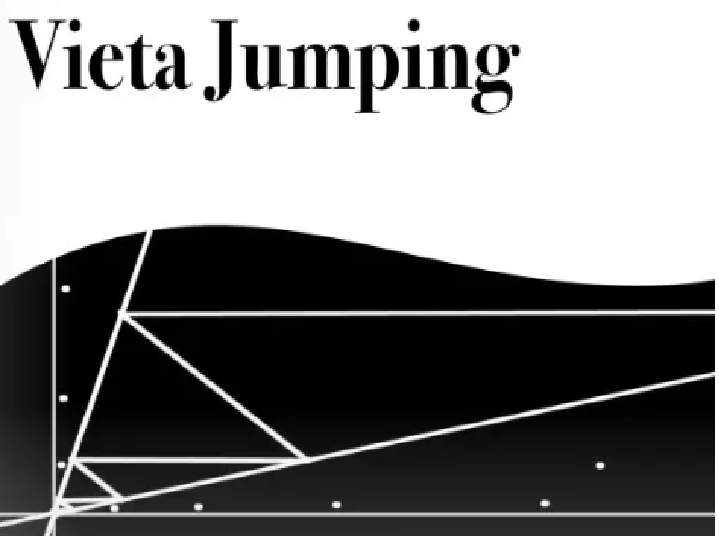
\includegraphics[scale=0.5]{images/vieta_jumping.png}
\end{center}

Vieta jumping is, however, more than just a cool way to solve olympiad problems--it also offers us a glimpse into the inner working of algebraic number theory and the interconnectedness of mathematics. There is no "purely" geometric or algebraic problem, rather every problem can fall in every category. (Indeed, the problem we did can also be about finding hyberbolas in the Cartesian Plane--see if you can reframe it to see why!)
\end{document}